\chapter*{misc}\addcontentsline{toc}{chapter}{misc}

Unsorted miscellaneous functions.

\HCode{<hr>}
System

\begin{quote}
\noindent
\hyperlink{acquire}{acquire} - search a variable in callers  \\
\hyperlink{clear}{clear},\hyperlink{clearglobal}{clearglobal} - removes variables from current or global environnement  \\
\end{quote}


\HCode{<hr>}
Programming

\begin{quote}
\noindent
\hyperlink{parse_dim_arg}{parse\_dim\_arg} - parse a string or number corresponding to a dimensional argument \\
\end{quote}


\HCode{<hr>}
Logical operators

\begin{quote}
\noindent
\hyperlink{and}{and} - logical and operator \\
\hyperlink{or}{or} - logical or operator \\
\hyperlink{not}{not} - logical not operator \\
\end{quote}

\HCode{<hr>}
Logical operator (Matlab compatibility)

\begin{quote}
\noindent
\hyperlink{any}{any} - checks if any element is nonzero or true  \\
\hyperlink{all}{all} - checks if all elements are nonzero or true \\
\end{quote}

\HCode{<hr>}
Coordinates transformation functions

\begin{quote}
\noindent
\hyperlink{sph2cart}{sph2cart},\hyperlink{cart2sph}{cart2sph} -
cartesian to spherical coordinates transformations functions \\
\end{quote}


\HCode{<hr>}
Special mathematical functions

\begin{quote}
\noindent
\hyperlink{bincoeff}{bincoeff} - {binomial coefficients}\\
\hyperlink{digamma}{digamma} - {logarithmic derivative of the gamma function}
\hyperlink{erfcx}{erfcx} - {The scaled complementary error function.}\\
\hyperlink{erfc}{erfc} - {The complementary error function.}\\
\hyperlink{erf}{erf} - {The error function.}\\
\hyperlink{gamma}{gamma} - {Gamma function}\\
\hyperlink{hypot}{hypot} - {length of hypotenuse.}\\
\hyperlink{legendre}{legendre} - associated legendre function\\
\hyperlink{lngamma}{lngamma} - {Logarithm of gamma function}\\
\end{quote}

\HCode{<hr>}
Polynomial

\begin{quote}
\noindent
\hyperlink{horner}{horner} - polynomial evaluation or composition \\
\hyperlink{hornerm}{hornerm} - substituting matrix in polynomial indeterminate \\
\hyperlink{cofactors}{cofactors} - gcd and cofactors of polynomials \\
\hyperlink{epdiv_fft}{epdiv\_fft} - {polynomial division using fft}\\
\hyperlink{epdiv_lsq}{epdiv\_lsq} - {polynomial division using least square linear solver}\\
\hyperlink{epdiv_gko}{epdiv\_gko} - { polynomial division using displacement solvers}\\
\hyperlink{repfreq}{repfreq} - {frequency response} \\
\end{quote}


\HCode{<hr>}
Geometry

\begin{quote}
\noindent
\hyperlink{convhull2d}{convhull2d} - {convex hull of a set of 2d-points}\\
\end{quote}

% -*- mode: latex -*-

\mansection{acquire}
\begin{mandesc}
  \short{acquire}{search a variable in callers} \\
\end{mandesc}

% -- Calling sequence section
\begin{calling_sequence}
\begin{verbatim}
y = acquire(name);
\end{verbatim}
\end{calling_sequence}
% -- Parameters
\begin{parameters}
  \begin{varlist}
    \vname{name}: a string giving the name of symbol to search.
    \vname{y} : a nsp object.
  \end{varlist}
\end{parameters}

\begin{mandescription}
  This function is used to copy in the current frame a variable found in callers 
  with the given name. 
\end{mandescription}

\begin{examples}
  \begin{program}\HCode{x=1:3;\Hnewline
      function y=f(n)\Hnewline
        if n >= 10 then y=acquire('x'); \Hnewline
	else y=f(n+1);\Hnewline
	end \Hnewline
      endfunction \Hnewline
      \Hnewline
      y=f(0);}
  \end{program}
\end{examples}

\begin{manseealso}
  \manlink{resume}{resume}  
\end{manseealso}

% -- Authors
\begin{authors}
  Jean-Philippe Chancelier
\end{authors}

% -*- mode: latex -*-

\mansection{clear}

\begin{mandesc}
  \short{clear}{remove variables from current environment} \\
  \short{clearglobal}{remove variables from global environment} 
\end{mandesc}
\index{clear}\label{clear}
\index{clearglobal}\label{clearglobal}
%-- Calling sequence section
\begin{calling_sequence}
\begin{verbatim}
  clear name1,...,namen;
  clear ;
  clear('name1',...,'namen');
  clear();
  clearglobal name1,...,namen;
  clearglobal ;
  clearglobal('name1',...,'namen');
  clearglobal();
\end{verbatim}

\end{calling_sequence}

\begin{mandescription}
  The \verb+clear+ (resp. \verb+clearglobal+) is used to remove (unprotected) variables given by their names 
  form the current (resp. the global) environment. If no argument is given to the command then all the 
  variables current (resp global) are removed. 
\end{mandescription}
%-- see also
\begin{manseealso}
  \manlink{who}{who}  
\end{manseealso}


% -*- mode: latex -*-

\mansection{parse\_dim\_arg}
\begin{mandesc}
 \shortunder{parse\_dim\_arg}{parse_dim_arg}{parse a string or number corresponding to a dimensional argument}
\end{mandesc}
% -- Calling sequence section
\begin{calling_sequence}
\begin{verbatim}
 rep = parse_dim_arg( dim_arg, names=[arg_name,func_name])  
\end{verbatim}
\end{calling_sequence}
% -- Parameters
\begin{parameters}
  \begin{varlist}
    \vname{dim_arg}: a string choosen among  \verb+'M'+, \verb+'m'+, \verb+'*'+, \verb+'full'+, \verb+'FULL'+, \verb+'row'+,
    \verb+'ROW'+, \verb+'col'+, \verb+'COL'+ or an non ambiguous abbreviation or an integer.
    \vname{names=[arg_name,func_name]}: optional named argument, a string matrix with 2 strings.
    \vname{rep}: an integer (0 for full, 1 for row, 2 for column, -2 for matlab compatibility flag).
  \end{varlist}
\end{parameters}
\begin{mandescription}
  This function could be useful to parse a ``dimensional argument'' (like in 
the functions sum, prod, ...) which generally indicates the dimension along which 
an operation must be done. In nsp this kind of argument could be either a string
or an integer and this function returns the corresponding integer:  

\begin{tabular}{|r|l|l|}
\hline
integer & equivalent strings & comment \\
\hline
0       & \verb+"full"+, \verb+"FULL"+, \verb+"*"+  &  operation along all the matrix (considered as a big vector) \\
1       & \verb+"row"+, \verb+"ROW"+                &  operation along all the first dimension \\
2       & \verb+"col"+, \verb+"COL"+                &  operation along all the second dimension \\
-2      & \verb+"m"+, \verb+"M"+                    &  flag for matlab compatibility \\
\hline
\end{tabular}
 
In case of a string, the function tests if it is in the set of
valid strings or if it corresponds to a non ambiguous abbreviation. In case of a number
the function tests if it is an integer larger than or equal to -2. If the test
fails, an error is setted with an error message. To have a more
meaningful message you can provide the optional argument 
\verb+names=[arg_name,func_name]+.
\end{mandescription}

% --example 
\begin{examples}

\begin{Verbatim}
function mu = freqmean(x,freq,dim=0)
   dim = parse_dim_arg(dim,names=["dim","freqmean"])
   if dim == -1 || dim > 2 then
      error("Error: unsupported dim flag")
   elseif dim == -2 then
      if isvector(x) then, dim = 0, else, dim = 1, end
   end
   mu = sum( x.*freq, dim )./ sum( freq, dim )
endfunction
x = [1, 2, 2.5, 4, 9; 5, -1, 0, 1, -5]
f = [1, 9, 2,   1, 2; 3,  2, 1, 1,  4]
mu = freqmean(x,f,dim="m")
mu = freqmean(x,f,dim=2)
mu = freqmean(x,f,dim="c")
mu = freqmean(x,f,dim=-3)  // should raise an error
mu = freqmean(x,f,dim=3)  // should raise an error
\end{Verbatim}
\end{examples}

% -- see also
\begin{manseealso}
\manlink{is_string_in_array}{is_string_in_array}
\end{manseealso}

\begin{authors}
  Bruno Pincon
\end{authors}



% -*- mode: latex -*-
\mansection{and, or}
\begin{mandesc}
  \short{and}{logical AND function or operator}\\
  \short{or}{logical OR function or operator}
\end{mandesc}

%-- Calling sequence section
\begin{calling_sequence}
\begin{verbatim}
  C = and(A)
  C = and(A,dim=dimarg) (equivalently C = and(A,dimarg))
  C = A & B (equivalently C = and(A,B))
  C = A && B 
  C = or(A)
  C = or(A,dim=dimarg) (equivalently or(A,dimarg))
  C = A | B (equivalently C = or(A,B))
  C = A || B 
\end{verbatim}
\end{calling_sequence}
% -- Parameters
\begin{parameters}
  \begin{varlist}
    \vname{A,B,C}: boolean matrices. 
    \vname{dimarg}: a string (\verb!'*'!,or \verb!'r'!,or \verb!'c'!) or an integer which defines 
    a dimension along which the boolean AND or OR operation is performed. 
  \end{varlist}
\end{parameters}

\begin{mandescription}
  \begin{itemize} 
  \item \itemdesc{and}
  \begin{itemize} 
  \item \verb!and(A)! is the logical AND of the elements of the boolean matrix \verb!A!. 
    \verb!and(A)! returns \verb!%t! iff all entries of \verb!A! are \verb!%t!. 
  \item \verb!y=and(A,dim='r')! (equivalently, \verb!y=and(A,'r')!,\verb!y=and(A,dim=1)! or \verb!y=and(A,1)!) 
    returns in \verb!y! a row vector such that \verb!y(j)= and(A(i,j),i=1,m)!). 
    \verb!y=and(A,dim='c')! (or, equivalently, \verb!y=and(A,dim=2)!) returns in \verb!y! a colum vector 
    such that \verb!y(i)= and(A(i,j),j=1,n)!)).
  \item \verb!A & B! or \verb!and(A,B)! gives the element-wise logical AND
    of the booleans matrices \verb!A! and  \verb!B!. The two matrices must have the same size 
    with the usual promotion of single booleans (\verb!1x1! matrices). 
  \item \verb!A && B! performs a sequential AND ; this is the same than 
    the element-wise logical AND but when $A(i,j)$ is false, the result $C(i,j)$
    is directly set to false, $B(i,j)$ being not evaluated.
  \end{itemize}
  \item \itemdesc{or}
  \begin{itemize} 
  \item \verb!or(A)! is the logical OR of the elements of the boolean matrix \verb!A!. 
    \verb!or(A)! returns \verb!%t! iff at least one entry of \verb!A! is \verb!%t!. 
  \item \verb!y=or(A,dim='r')! (equivalently, \verb!y=or(A,'r')!,\verb!y=or(A,dim=1)! or \verb!y=or(A,1)!) 
    returns in \verb!y! a row vector such that \verb!y(j)= or(A(i,j),i=1,m)!). 
    \verb!y=or(A,dim='c')! (equivalently, \verb!y=or(A,dim=2)!) returns in \verb!y! a colum vector 
    such that \verb!y(i)= or(A(i,j),j=1,n)!)).
  \item \verb!A | B! (equivalently \verb!or(A,B)!) gives the element-wise logical  OR
    of the booleans matrices \verb!A! and  \verb!B!. The two matrices must have the same size 
    with the usual promotion of single booleans (\verb!1x1! matrices). 
  \item \verb!A || B! performs a sequential OR ; this is the same than 
    the element-wise logical OR but when $A(i,j)$ is true, the result $C(i,j)$
    is directly set to true, $B(i,j)$ being not evaluated.
  \end{itemize} 
\end{itemize}

\end{mandescription}

%--example 
\begin{examples}
\paragraph{AND basic examples}
  \begin{program}\HCode{A = [\%t, \%f, \%t; \%t,\%t, \%f; \%t,\%t, \%t]\Hnewline
    and(A)\Hnewline
    and(A,dim=1)\Hnewline
    and(A,dim=2)\Hnewline
    B = rand(3,3) < 0.5\Hnewline
    A & B\Hnewline
    A }\verb+&&+\HCode{ B\Hnewline
    // difference between & and }\verb+&&+\HCode{\Hnewline
    i = 0;\Hnewline
    x = rand(1,3)\Hnewline
    bool = i > 0 }\verb+&&+\HCode{ x(i) < 0.5 // the 2d expression is not evaluated\Hnewline
    bool = i > 0 & x(i) < 0.5 // the 2d expression is evaluated and so raise an error}
  \end{program}

\paragraph{OR basic examples}
  \begin{program}\HCode{A = [\%t, \%f, \%f; \%t,\%t, \%f; \%f,\%f, \%f]\Hnewline
    or(A)\Hnewline
    or(A,dim=1)\Hnewline
    or(A,dim=2)\Hnewline
    B = rand(3,3) < 0.5\Hnewline
    A | B\Hnewline
    A || B\Hnewline
    // difference between | and || \Hnewline
    i = 0;\Hnewline
    x = rand(1,3)\Hnewline
    bool = i == 0 || x(i) < 0.5 // the 2d expression is not evaluated\Hnewline
    bool = i == 0 || x(i) < 0.5 // the 2d expression is evaluated and so raise an error}
  \end{program}

\end{examples}

%-- see also
\begin{manseealso}
  \manlink{not}{not},\manlink{any}{any}, \manlink{all}{all}  

\end{manseealso}


% -*- mode: latex -*-
\mansection{not}
\begin{mandesc}
  \short{not}{logical NOT function or operator}
\end{mandesc}

%-- Calling sequence section
\begin{calling_sequence}
\begin{verbatim}
  B = ~A  (equivalently B = not(A))
\end{verbatim}
\end{calling_sequence}
% -- Parameters
\begin{parameters}
  \begin{varlist}
    \vname{A,B}: boolean matrices. 
  \end{varlist}
\end{parameters}

\begin{mandescription}
  Returns a boolean matrix (says \verb+B+) of same dimensions than \verb+A+ by applying
  the logical NOT to each element (B(i,j) = not(A(i,j)).
\end{mandescription}

%--example 
\begin{examples}
  \begin{program}\HCode{A = [\%t, \%f, \%t; \%t,\%t, \%f; \%t,\%t, \%t]\Hnewline
   }\verb+~+\HCode{A}
  \end{program}

\end{examples}

%-- see also
\begin{manseealso}
  \manlink{and}{and}, \manlink{or}{or},\manlink{any}{any}, \manlink{all}{all}  
\end{manseealso}


% -*- mode: latex -*-

\mansection{cartesian to spherical coordinates transformations}
\begin{mandesc}
   \short{cart2sph}{cartesian to spherical coordinates}\\
   \short{sph2cart}{spherical to cartesian coordinates}
\end{mandesc}

%-- Calling sequence section
\begin{calling_sequence}
\begin{verbatim}
 [theta, phi, r] = cart2sph(x, y, z)
 [theta, phi, r] = cart2sph(x, y, z, colat=%t)
 [x, y, z] = sph2cart(theta, phi, r)
 [x, y, z] = sph2cart(theta, phi, r, colat=%t)
\end{verbatim}
\end{calling_sequence}

%-- Parameters
\begin{parameters}
  \begin{varlist}
   \vname{x, y, z}: real vectors or matrices of same dimensions
   \vname{colat}: boolean optional named argument (default is \%f)
   \vname{theta, phi, r}: real vectors or matrices
  \end{varlist}
\end{parameters}

\begin{mandescription}
  Computes correspondance between cartesian coordinates $(x,y,z)$ and spherical
  coordinates $(\theta,\phi,r)$ :
\begin{itemize}
\item $\theta$ the azimuth angle (in $[0,2\pi)$)
\item $\phi$ the latitude (or elevation) angle by default or
      when \verb+colat=%f+ (here $\phi$ is in $[-pi/2,pi/2]$) or 
      the colatitude angle when \verb+colat=%t+ (in this case  $\phi$ is in $[0,pi]$)
\item and $r$ the euclidian distance between $O=(0,0,0)$ and $M=(x,y,z)$.
\end{itemize}

$$
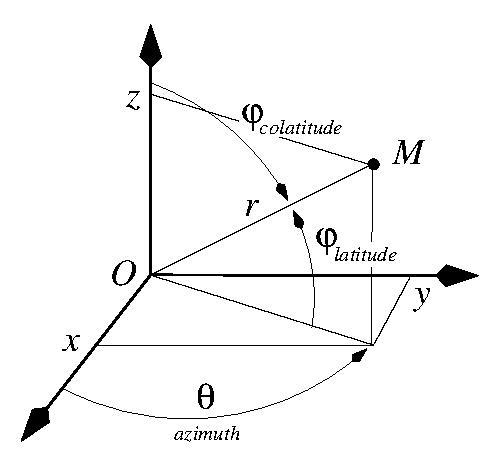
\includegraphics[width=8cm]{spherical} 
$$

We have the relations:
$$
\mbox{with } \varphi \mbox{ latitude}: 
\left\{\begin{array}{l}
x = r \cos(\theta) \cos(\varphi) \\
y = r \sin(\theta) \cos(\varphi) \\
z = r \sin(\varphi)
\end{array}\right.
\mbox{                  and with } \varphi \mbox{ colatitude}: 
\left\{ \begin{array}{l}
x = r \cos(\theta) \sin(\varphi) \\
y = r \sin(\theta) \sin(\varphi) \\
z = r \cos(\varphi)
\end{array} \right.
$$


\paragraph{remark}
One or two input argument(s) could be a scalar.
  
\end{mandescription}

%--example 
\begin{examples}
\begin{program}\HCode{[theta,phi,r]=cart2sph(1,1,sqrt(2))\Hnewline
// theta and phi must be equal to pi/4 and r must be equal to 2\Hnewline
[x,y,z] = sph2cart(theta, phi, r)\Hnewline
// x, y and z should be equal or very near 1, 1 and sqrt(2)}
\end{program}
\end{examples}



% -*- mode: latex -*-

\mansection{legendre}
\begin{mandesc}
   \short{legendre}{associated Legendre functions}
\end{mandesc}

%-- Calling sequence section
\begin{calling_sequence}
\begin{verbatim}
 y = legendre(n,m,x [,normflag]) 
\end{verbatim}
\end{calling_sequence}

%-- Parameters
\begin{parameters}
  \begin{varlist}
   \vname{n} : non negative integer or vector of non negative integers regularly spaced with increment equal to 1
   \vname{m} : non negative integer or vector of non negative integers regularly spaced with increment equal to 1
   \vname{x} : real vector (elements of $x$ must be in $[-1,1]$)
   \vname{normflag} : (optional) scalar string
  \end{varlist}
\end{parameters}

\begin{mandescription}
  When $n$ and $m$ are scalars, \verb!legendre(n,m,x)! evaluates the associated Legendre 
  function $Pnm(x)$ at all the elements of $x$. The definition used is :
$$  
P_{nm}(x) = (-1)^m \left(1 - x^2 \right)^{m/2} \frac{d^m}{dx^m} P_n (x)
$$
where $Pn$ is the Legendre polynomial of degree $n$. So 
\verb!legendre(n,0,x)! evaluates the Legendre polynomial $Pn(x)$ at all 
the elements of $x$. 
  
When the normflag is equal to "norm" you get a normalized version (without
the \verb!(-1)^m! factor) :
$$
 P_{nm}^{norm}(x) = \sqrt{\frac{(2n+1) (n-m)!}{2 (n+m)!}} \left(1 - x^2 \right)^{m/2} \frac{d^m}{dx^m} P_n (x)
$$
which is useful to compute spherical harmonic functions (see Example 3).
  
For efficiency, one of the two first arguments may be a vector, for instance
\verb!legendre(n1:n2,0,x)! evaluates all the Legendre polynomials of
degree $n_1, n_1+1, ..., n_2$ at the elements of $x$ and
\verb!legendre(n,m1:m2,x)! evaluates all the Legendre associated 
functions $P_{nm}$ for $m=m_1, m_1+1, ..., m_2$ at $x$.

\paragraph{Output format}

In any case, the format of \verb!y! is \verb+max(length(n),length(m)) x length(x)+
with :
\begin{verbatim}
       y(i,j) = P(n(i),m;x(j))   if n is a vector
       y(i,j) = P(n,m(i);x(j))   if m is a vector
       y(1,j) = P(n,m;x(j))      if both n and m are scalars
\end{verbatim}
so that $x$ is preferably a row vector but any \texttt{mx x nx} matrix
is excepted and considered as an \texttt{1 x (mx * nx)} matrix, reshaped
following the column order.
  
\end{mandescription}

%--example 
\begin{examples}
\paragraph{example 1} plot the 6 first Legendre polynomials:
\begin{program}\HCode{x = linspace(-1,1,200)';\Hnewline
y = legendre(0:5, 0, x);\Hnewline
xbasc()\Hnewline
plot2d(x,y', leg="p0@p1@p2@p3@p4@p5@p6")\Hnewline
xtitle("the 6 th first Legendre polynomials")}
\end{program}

\paragraph{example 2} plot of the associated Legendre functions of degree 5 
\begin{program}\HCode{x = linspace(-1,1,200)';\Hnewline
y = legendre(5, 0:5, x, "norm");\Hnewline
xbasc()\Hnewline
plot2d(x,y', leg="p5,0@p5,1@p5,2@p5,3@p5,4@p5,5")\Hnewline
xtitle("the (normalised) associated Legendre functions of degree 5")}
\end{program}

\paragraph{example 3} plot spherical harmonics
\begin{program}\HCode{// define Ylm functions\Hnewline
function [y] = harm_sph_Y(l,m,phi,theta)\Hnewline
   pl = legendre(l, abs(m), cos(phi), "norm")\Hnewline
   pl.redim[size(phi)]\Hnewline
   if m >= 0 then\Hnewline
      y = (-1)^m/(sqrt(2*\%pi))*exp(\%i*m*theta).*pl\Hnewline
   else\Hnewline
      y = 1/(sqrt(2*\%pi))*exp(\%i*m*theta).*pl\Hnewline
   end      \Hnewline
endfunction\Hnewline
// la suite un autre jour}
\end{program}

\end{examples}

%-- Authors
\begin{authors}
Smith, John M. (code dxlegf.f from Slatec), B. Pincon (nsp interface + slight modifs on dxlegf.f) 
\end{authors}


% -*- mode: latex -*-
\mansection{any}
\begin{mandesc}
  \short{any}{checks if any element is nonzero or true} 
\end{mandesc}
\begin{calling_sequence}
\begin{verbatim}
 B= any(A [,dim=val])
 B= any(A [,val])
\end{verbatim}
\end{calling_sequence}
% -- Parameters
\begin{parameters}
  \begin{varlist}
    \vname{A}:  matrix of numbers or booleans 
    \vname{B}: a boolean matrix 
    \vname{dim=val} optional argument chosen among the possible strings '*', 
    'full', 'FULL', 'row', 'ROW', 'col', or 'COL'  or an non ambiguous abbreviation or an 
    integer as follows $0$ for 'full', $1$ for 'row', $2$ for 'column'.
  \end{varlist}
\end{parameters}

\begin{mandescription}
  \verb!any! checks if any elements are nonzero (resp. are true) when a matrix of numbers (resp. of booleans) 
  is given as argument. The size of the result and the elements of the matrix taken in consideration depends 
  on the optional argument \verb!dim! as follows~:
  \begin{itemize}
  \item \verb!'*'! The answer is scalar and equal to true if any element of the matrix \verb!A!
    are nonzero (resp. are true).
  \item \verb!'r'! The answer is a row vector which contains true value when any element of 
    the corresponding column of the matrix is nonzero (resp. is true). 
  \item \verb!'c'! The answer is a column vector which contains true value when any element of 
    the corresponding row of the matrix is nonzero (resp. is true).
  \end{itemize}
  The default behaviour is to follow the Matlab rules i.e the mode is by default \verb!'r'! 
  for a matrix except for row vectors for which the defaultmode is \verb!'*'!. 
  This mode should also be obtained by \verb!'m'! in a near future. 
\end{mandescription}
%-- see also
\begin{manseealso}
  \manlink{all}{all}, \manlink{and}{and}, \manlink{or}{or}, \manlink{not}{not}
\end{manseealso}
%-- Authors


% -*- mode: latex -*-
\mansection{all}
\begin{mandesc}
  \short{all}{checks if all elements are nonzero or true} 
\end{mandesc}

\begin{calling_sequence}
\begin{verbatim}
 B= all(A [,dim=val])
 B= all(A [,val])
\end{verbatim}
\end{calling_sequence}
% -- Parameters
\begin{parameters}
  \begin{varlist}
    \vname{A}:  matrix of numbers or booleans 
    \vname{B}: a boolean matrix 
    \vname{val}: optional argument chosen among the possible strings '*', 
    'full', 'FULL', 'row', 'ROW', 'col', or 'COL'  or an non ambiguous abbreviation or an 
    integer as follows $0$ for 'full', $1$ for 'row', $2$ for 'column'.
  \end{varlist}
\end{parameters}

\begin{mandescription}
  \verb!all! checks if elements are nonzero (resp. are true) when a matrix of numbers (resp. of booleans) 
  is given as argument. The size of the result and the number of arguments taken in consideration depends 
  on the optional argument \verb!dim! as follows:
  \begin{itemize}
  \item \verb!'*'! The answer is scalar and true if all the elements are nonzero (resp. are true).
  \item \verb!'r'! The answer is a row vector which contains true value when all the elements of 
    the corresponding column of the matrix are  nonzero (resp. are true). 
  \item \verb!'c'! The answer is a column vector which contains true value when all the elements of 
    the corresponding row of the matrix are  nonzero (resp. are true).
  \end{itemize}
  The default behaviour is to follow the Matlab rules i.e the mode is by default \verb!'r'! 
  for a matrix except for row vectors for which the defaultmode is \verb!'*'!. 
  This mode should also be obtained by \verb!'m'! in a near future. 
\end{mandescription}
%-- see also
\begin{manseealso}
  \manlink{any}{any}, \manlink{and}{and}, \manlink{or}{or}, \manlink{not}{not}
\end{manseealso}
%-- Authors




% -*- mode: latex -*-
\mansection{horner}
\begin{mandesc}
  \short{horner}{polynomial evaluation} \\ % 
\end{mandesc}
%-- Calling sequence section
\begin{calling_sequence}
\begin{verbatim}
  R=horner(P,Q, vdim=%f, ttmode=%f)
\end{verbatim}
\end{calling_sequence}
%-- Parameters
\begin{parameters}
  \begin{varlist}
    \vname{P}: polynomial matrix
    \vname{Q}: a polynomial or numerical matrix
    \vname{vdim, ttmode}: optional named boolean arguments.
    \vname{R}: a cell if \verb!ttmode! is false and a 
    polynomial or a numerical matrix if \verb!ttmode! is true.
  \end{varlist}
\end{parameters}
\begin{mandescription}
  Evaluates the polynomial matrix \verb!P! at values given by \verb!Q! 
  using the Horner algorithm. When \verb!Q! is a 
  numerical matrix the Horner algorithm is a builtin function 
  and when \verb!Q! is a  polynomial matrix the computation is 
  performed with a library nsp function. 
  
  \begin{itemize} 
  \item When \verb!ttmode! is true then the performed operation is a term to term 
    horner which implies that both matrices must have same dimensions (with 
    the usual convention that \verb!1x1! matrices are promoted 
    to any dimensions). The returned result, \verb!R! is a polynomial matrix if 
    \verb!Q! is a polynomial matrix or a numerical matrix if \verb!Q! is numeric 
    which is given by \verb!R(i,j) = horner(P(i,j),Q(i,j)\verb!
  \item When \verb!ttmode! is false the returned value, \verb!R! is a cell matrix 
    \begin{itemize}
    \item if \verb!vdim! is false the cell matrix has same dimension 
      as \verb!P! and the cell element \verb!(i,j)! is the polynomial or 
      numerical matrix \verb!P(i,j)(Q)!. 
    \item if \verb!vdim! is true the cell matrix has same dimension 
      as \verb!Q! and the cell element \verb!(i,j)! is the polynomial
      or numerical matrix \verb!P(Q(i,j))!.
    \end{itemize}
  \end{itemize}
\end{mandescription}
%--example 
\begin{examples}
  \begin{itemize}
  \item \verb!ttmode=%f!
    \begin{mintednsp}{nsp}
      p=m2p(1:3);
      q=m2p(1:2);
      r=testmatrix('magic',3);
      R=horner([p,q],r); // a 1x2 cell 
      R1=horner([p,q],r,vdim=%t); // a 3x3 cell
      A=ce2m(R1,indice=1); // a 3x3 matrix 
      B=ce2m(R1,indice=2); // a 3x3 matrix 
      R.equal[{A,B}]  // recovering R from R1.
    \end{mintednsp}
  \item \verb!ttmode=%t!
    \begin{mintednsp}{nsp}
      P = ce2p({1:2,1;2,[1,-1]})
      Q1 = ce2p({1,[1,4];[0,1],[1,-1]})
      R1=horner(P,Q1,ttmode=%t);
      
      Q2 =[1,2;3,7];
      R2=horner(P,Q2,ttmode=%t);
    \end{mintednsp}
  \end{itemize}
\end{examples}

%-- see also
%\begin{manseealso}
%\end{manseealso}

% -*- mode: latex -*-
\mansection{cofactors}
\begin{mandesc}
  \short{cofactors}{gcd and cofactors of polynomials}\\ % @mandesc@
\end{mandesc}
%-- Calling sequence section
\begin{calling_sequence}
\begin{verbatim}
 [g,p,q]=cofactors(u,v,td, iter=%t|%f,ftol=1.e-14)   
\end{verbatim}
\end{calling_sequence}
%-- Parameters
\begin{parameters}
  \begin{varlist}
    \vname{u,v}: polynomials. 
    \vname{td}: an integer. 
    \vname{g,p,q}: polynomials.
  \end{varlist}
\end{parameters}
\begin{mandescription}
  This function is used by the function \verb+gcd+. 
  Given an integer \verb+td+ as a tentative gcd degree, the function \verb+cofactors+ 
  computes the two cofactors \verb+p+ and \verb+q+ such that \verb+q*u - p*v=0+ and a 
  polynomial \verb+g+ of \verb+td+ degree (using \verb+epdiv_lsq+) such that:
\begin{verbatim}
     p*g - u = 0 
     q*g - v = 0
\end{verbatim} 
  If \verb+iter+ is true, iterative refinement is performed to minimize the euclidian 
  norm of \verb+(p*g - u,q*g - v)+ using the function \verb+fsolve_lsq+ \verb+ftol+ 
  being transmited to \verb+fsolve_lsq+. The 
  companion function which performs iterative refinement is called 
  \verb+cofactors_iter+. 
\end{mandescription}
%--example 
\begin{examples}
  \begin{Verbatim}
    x=poly(0);
    u=(1+x+x^3+x^4)*(1+6*x);
    v=(1+x+x^3+x^4)*(1+7*x);
    k=4; // tentative degree 
    [g,p,q]=cofactors(u,v,k,iter=%f)
    [norm( g*p -u ), norm(g*q -v )]
    [g,p,q]=cofactors(u,v,k)
    [norm( g*p -u ), norm(g*q -v )]
  \end{Verbatim}
\end{examples}
%-- see also
\begin{manseealso}
  \manlink{Pmat}{Pmat}, \manlink{epdiv\_lsq}{epdiv_lsq}
\end{manseealso}
%-- Author
\begin{authors}
  J.Ph Chancelier. 
\end{authors}


% -*- mode: latex -*-
\mansection{epdiv}
\begin{mandesc}
  \shortunder{epdiv\_fft}{epdiv_fft}{polynomial division using fft}\\ 
  \shortunder{epdiv\_lsq}{epdiv_lsq}{polynomial division using least square linear solver}\\ 
  \shortunder{epdiv\_gko}{epdiv_gko}{polynomial division using displacement solvers}
\end{mandesc}
%-- Calling sequence section
\begin{calling_sequence}
\begin{verbatim}
 [q]=epdiv_fft(u,v)
 [q]=epdiv_lsq(u,v)
 [q]=epdiv_gko(u,v)
\end{verbatim}
\end{calling_sequence}
%-- Parameters
\begin{parameters}
  \begin{varlist}
    \vname{u,v,q}: polynomials. 
  \end{varlist}
\end{parameters}
\begin{mandescription}
  these functions compute the result of the division of polynomial \verb+u+ by 
  \verb+v+ assuming that \verb+u+ is exactly divisible by \verb+v+
\end{mandescription}
%--example 
\begin{examples}
  \begin{Verbatim}
  x=poly(0);
  p=(1+x)*(1+2*x)*(1+5*x);
  q=(1+2*x);
  u=epdiv_fft(p,q);
  if norm(p -q*u) > 1.e-10 then pause;end 
  u=epdiv_lsq(p,q);
  if norm(p -q*u) > 1.e-10 then pause;end 
  u=epdiv_gko(p,q);
  if norm(p -q*u) > 1.e-10 then pause;end 
  \end{Verbatim}
\end{examples}
%-- see also
\begin{manseealso}
  \manlink{Pmat}{Pmat} 
\end{manseealso}
%-- Author
\begin{authors}
  Paola Boito,  J.Ph Chancelier. 
\end{authors}


% -*- mode: latex -*-
% Copyright (C) CeCILL Inria (scilab)
% -*- mode: latex -*-
\mansection{repfreq}
\begin{mandesc}
  \short{repfreq}{frequency response} \\ % 
\end{mandesc}
%\index{repfreq}\label{repfreq}
%-- Calling sequence section
\begin{calling_sequence}
\begin{verbatim}
 [frq,repf,split]= repfreq(n,d,fmin=,fmax=,step=,frq=)   
 [repf]=repfreq(n,d,fmin=,fmax=,step=,frq=)  
\end{verbatim}
\end{calling_sequence}
%-- Parameters
\begin{parameters}
  \begin{varlist}
    \vname{n,d}: two polynomial matrices of size \verb!nx1!
    \vname{fmin}: a real for minimal frequency bounds (in Hz) or \verb!sym!
    \vname{fmax}: a real for maximal frequency bounds (in Hz).
    \vname{step}: a real (logarithmic step) or a string \verb!'auto'!.
    \vname{frq}: a row vector or a \verb!nx1! matrix giving frequencies (in Hz).
    \vname{dom}: time domain \verb!'c'! or \verb!'d'! or a positive real (default \verb!'c'!).
    \vname{split}: vector of indexes of critical frequencies.
  \end{varlist}
\end{parameters}
\begin{mandescription}
  \verb!repfreq! returns the frequency response calculation of a linear system \verb!n/d! at frequencies. 

  The frequencies are given by the matrix \verb!frq! or computed from
  the bounds \verb!fmin! and \verb!fmax! (in Hz) and \verb!step! giving
  the ( logarithmic ) discretization step which is automatically adapted if
  (\verb!step='auto'!).
    
  \begin{description}
  \item[dom='c']: \verb!repf(k)=(n/d)(  2*%i*%pi*frq(k))! 
  \item[dom='d']]: \verb!repf(k)=(n/d)( 2*%i*%pi*dt*frq(k))! with \verb!dt=1! 
  \item[dom=x]]: \verb!repf(k)=(n/d)( 2*%i*%pi*dt*frq(k))! with \verb!dt=x! 
  \end{description}

  The vector \verb!frq! is splitted into regular parts with the \verb!split! vector i.e 
  \verb!frq(splitf(k):splitf(k+1)-1)! has no critical frequency. In other words, 
  the system \verb!n/d! has a pole in the range \verb![frq(splitf(k)),frq(splitf(k)+1)]! and 
  no poles outside.
\end{mandescription}
%--example 
% \begin{examples}
%   \begin{mintednsp}{nsp}
%   \end{mintednsp}
% \end{examples}
%-- see also
\begin{manseealso}
  \manlink{bode}{bode}
%  \manlink{freq}{freq} 
%  \manlink{calfrq}{calfrq} 
  \manlink{horner}{horner} 
  \manlink{nyquist}{nyquist} 
%  \manlink{dbphi}{dbphi}  
\end{manseealso}
%-- Author
\begin{authors}
  Serge Steer
\end{authors}


% -*- mode: latex -*-
\mansection{bincoeff}
\begin{mandesc}
  \short{bincoeff}{binomial coefficients}\\
\end{mandesc}
%-- Calling sequence section
\begin{calling_sequence}
\begin{verbatim}
  c = bincoeff(n,k);
\end{verbatim}
\end{calling_sequence}
%-- Parameters
\begin{parameters}
  \begin{varlist}
    \vname{n,k}: real vectors or matrices of the same size.
  \end{varlist}
\end{parameters}

\begin{mandescription}
  This function returns in \verb+c(i)+ the binomial coefficients 
  of \verb+n(i)+ and \verb+k(i)+ defined by: 
\[
   \operatorname{bincoeff}(n,k) = \binom{n}{k} := \frac{n!}{k! (n-k)!}
\]
\end{mandescription}
% -- Authors
\begin{examples}

\begin{mintednsp}{nsp}
  N=10; n= N*ones(1,N+1),k=0:N;
  c=bincoeff(n,k);
  d= gamma(n+1) ./ (gamma(k+1).*gamma(n-k+1));
  max(abs(c-d))
\end{mintednsp}

\paragraph{we check the following identity}
\[
(1+x)^n = \sum_{k=0}^n \binom{n}{k} x^k
\]
\begin{mintednsp}{nsp}
  n=10;
  c=bincoeff(n*ones(1,n+1),0:n);
  x=2; 
  y=sum( c .* x.^(0:n));
  y == (1+x)^n
\end{mintednsp}

\end{examples}

% -*- mode: latex -*-
\mansection{convhull2d}
\begin{mandesc}
  \short{convhull2d}{convex hull of a set of 2d-points}\\
\end{mandesc}
%-- Calling sequence section
\begin{calling_sequence}
\begin{verbatim}
  I=convhull2d(x,y);
\end{verbatim}
\end{calling_sequence}
%-- Parameters
\begin{parameters}
  \begin{varlist}
    \vname{x,y}: two vectors or matrices of the same size
    \vname{I}: a vector of indices 
  \end{varlist}
\end{parameters}

\begin{mandescription}
  The function \verb+convhull2d+ computes the convex hull of 
  a set of 2d points given by \verb!(x(.),y(.))!. The convex 
  hull is returned as a vector of indices to be used to extract 
  the convex hull from the given points. That is, the convex hull 
  is given by the points \verb!(x(I(.)),y(I(.)))!.
\end{mandescription}
%--example 
\begin{examples}
  \begin{mintednsp}{nsp}
    x=rand(1,50);
    y=rand(1,50);
    I=convhull2d(x,y);
    rect=[-0.2,-0.2,1.2,1.2]
    plot2d(x(I),y(I),line_color=3,rect=rect);
    plot2d(x,y,line_color=-2,mark=1,rect=rect);
  \end{mintednsp}
\end{examples}
% -- see also
% \begin{manseealso}
%   \manlink{indexing arrays}{indexing arrays}
% \end{manseealso}


% -*- mode: latex -*-
\mansection{erf,erfc,erfcx}
\begin{mandesc}
  \short{erf}{The error function.}\\
  \short{erfc}{The complementary error function.}\\
  \short{erfcx}{The scaled complementary error function.}\\
\end{mandesc}
%-- Calling sequence section
\begin{calling_sequence}
\begin{verbatim}
  y = erf(x);
  y = erfc(x);  
  y = erfcx(x);  
\end{verbatim}
\end{calling_sequence}
%-- Parameters
\begin{parameters}
  \begin{varlist}
    \vname{x}: real vector or matrix
    \vname{y}: real vector or matrix (of same size than x)
  \end{varlist}
\end{parameters}

\begin{mandescription}
  The error function \verb+erf+ is defined by:
\[
  \operatorname{erf}(x) :=\frac{2}{\sqrt{\pi}} \int_0^x \exp(-y^2) dy \,.
\]
  The complementary error function \verb+erfc+ is defined by:
\[
\operatorname{erfc}(x) := 1 - \operatorname{erf}(x) = \frac{2}{\sqrt{\pi}} \int_x^{\infty} \exp(-y^2)dy \,.
\]
The scaled complementary error function \verb+erfcx+ is defined by:
\[
\operatorname{erfcx}(x) := \exp(x^2) \operatorname{erfc}(x)\,.
\]
\end{mandescription}

%--example 
\begin{examples}
\begin{mintednsp}{nsp}
  function y=f(x); y = exp(-x.^2);endfunction;
  x=2;intg(0,x,f)*2/sqrt(%pi) - erf(x);
\end{mintednsp}
\end{examples}
%-- see also
%\begin{manseealso}
%\manlink{indexing arrays}{indexing arrays}
%\end{manseealso}


% -*- mode: latex -*-
\mansection{erf,erfc,erfcx}
\begin{mandesc}
  \short{erf}{The error function.}\\
  \short{erfc}{The complementary error function.}\\
  \short{erfcx}{The scaled complementary error function.}\\
\end{mandesc}
%-- Calling sequence section
\begin{calling_sequence}
\begin{verbatim}
  y = erf(x);
  y = erfc(x);  
  y = erfcx(x);  
\end{verbatim}
\end{calling_sequence}
%-- Parameters
\begin{parameters}
  \begin{varlist}
    \vname{x}: real vector or matrix
    \vname{y}: real vector or matrix (of same size than x)
  \end{varlist}
\end{parameters}

\begin{mandescription}
  The error function \verb+erf+ is defined by:
\[
  \operatorname{erf}(x) :=\frac{2}{\sqrt{\pi}} \int_0^x \exp(-y^2) dy \,.
\]
  The complementary error function \verb+erfc+ is defined by:
\[
\operatorname{erfc}(x) := 1 - \operatorname{erf}(x) = \frac{2}{\sqrt{\pi}} \int_x^{\infty} \exp(-y^2)dy \,.
\]
The scaled complementary error function \verb+erfcx+ is defined by:
\[
\operatorname{erfcx}(x) := \exp(x^2) \operatorname{erfc}(x)\,.
\]
\end{mandescription}

%--example 
\begin{examples}
\begin{mintednsp}{nsp}
  function y=f(x); y = exp(-x.^2);endfunction;
  x=2;intg(0,x,f)*2/sqrt(%pi) - erf(x);
\end{mintednsp}
\end{examples}
%-- see also
%\begin{manseealso}
%\manlink{indexing arrays}{indexing arrays}
%\end{manseealso}


% -*- mode: latex -*-
\mansection{erf,erfc,erfcx}
\begin{mandesc}
  \short{erf}{The error function.}\\
  \short{erfc}{The complementary error function.}\\
  \short{erfcx}{The scaled complementary error function.}\\
\end{mandesc}
%-- Calling sequence section
\begin{calling_sequence}
\begin{verbatim}
  y = erf(x);
  y = erfc(x);  
  y = erfcx(x);  
\end{verbatim}
\end{calling_sequence}
%-- Parameters
\begin{parameters}
  \begin{varlist}
    \vname{x}: real vector or matrix
    \vname{y}: real vector or matrix (of same size than x)
  \end{varlist}
\end{parameters}

\begin{mandescription}
  The error function \verb+erf+ is defined by:
\[
  \operatorname{erf}(x) :=\frac{2}{\sqrt{\pi}} \int_0^x \exp(-y^2) dy \,.
\]
  The complementary error function \verb+erfc+ is defined by:
\[
\operatorname{erfc}(x) := 1 - \operatorname{erf}(x) = \frac{2}{\sqrt{\pi}} \int_x^{\infty} \exp(-y^2)dy \,.
\]
The scaled complementary error function \verb+erfcx+ is defined by:
\[
\operatorname{erfcx}(x) := \exp(x^2) \operatorname{erfc}(x)\,.
\]
\end{mandescription}

%--example 
\begin{examples}
\begin{mintednsp}{nsp}
  function y=f(x); y = exp(-x.^2);endfunction;
  x=2;intg(0,x,f)*2/sqrt(%pi) - erf(x);
\end{mintednsp}
\end{examples}
%-- see also
%\begin{manseealso}
%\manlink{indexing arrays}{indexing arrays}
%\end{manseealso}


% -*- mode: latex -*-
\mansection{gamma,lngamma,digamma}
\begin{mandesc}
  \short{gamma}{Gamma function}\\
  \short{lngamma}{Logarithm of gamma function}\\
  \short{digamma}{logarithmic derivative of the gamma function}
\end{mandesc}
%-- Calling sequence section
\begin{calling_sequence}
\begin{verbatim}
  y = gamma(x);
  y = lngamma(x);  
  y = digamma(x);  
\end{verbatim}
\end{calling_sequence}
%-- Parameters
\begin{parameters}
  \begin{varlist}
    \vname{x,y}: real vector or matrix
  \end{varlist}
\end{parameters}

\begin{mandescription}
  The function \verb+gamma+ is defined by: 
  \[
  \operatorname(gamma) := \int_0^{+\infty} \exp(-y)y^{x-1} dy \,.
  \]
  The function \verb+lngamma+ is defined by:
  \[
  \operatorname{lngamma}(x) := ln(x)\Gamma(x) \,.
  \]
  The function \verb+digamma+ (also known as the \verb+psi+ function) 
  is defined by:
  \[
  \operatorname{digamma}(x) := Gamma'(x)/Gamma(x)\,.
  \]  
\end{mandescription}
%--example 
\begin{examples}
\begin{mintednsp}{nsp}
  function y=f(x); y = exp(-x.^2);endfunction;
  x=2;intg(0,x,f)*2/sqrt(%pi) - gamma(x);
\end{mintednsp}

\begin{mintednsp}{nsp}
function y=f(x); y = digamma(x);endfunction;
a=0.1;b=4;
y= abs(intg(a,b,f) - (lngamma(b) -lngamma(a)))
\end{mintednsp}

\end{examples}
%-- see also
%\begin{manseealso}
%\manlink{indexing arrays}{indexing arrays}
%\end{manseealso}


% -*- mode: latex -*-
\mansection{gamma,lngamma,digamma}
\begin{mandesc}
  \short{gamma}{Gamma function}\\
  \short{lngamma}{Logarithm of gamma function}\\
  \short{digamma}{logarithmic derivative of the gamma function}
\end{mandesc}
%-- Calling sequence section
\begin{calling_sequence}
\begin{verbatim}
  y = gamma(x);
  y = lngamma(x);  
  y = digamma(x);  
\end{verbatim}
\end{calling_sequence}
%-- Parameters
\begin{parameters}
  \begin{varlist}
    \vname{x,y}: real vector or matrix
  \end{varlist}
\end{parameters}

\begin{mandescription}
  The function \verb+gamma+ is defined by: 
  \[
  \operatorname(gamma) := \int_0^{+\infty} \exp(-y)y^{x-1} dy \,.
  \]
  The function \verb+lngamma+ is defined by:
  \[
  \operatorname{lngamma}(x) := ln(x)\Gamma(x) \,.
  \]
  The function \verb+digamma+ (also known as the \verb+psi+ function) 
  is defined by:
  \[
  \operatorname{digamma}(x) := Gamma'(x)/Gamma(x)\,.
  \]  
\end{mandescription}
%--example 
\begin{examples}
\begin{mintednsp}{nsp}
  function y=f(x); y = exp(-x.^2);endfunction;
  x=2;intg(0,x,f)*2/sqrt(%pi) - gamma(x);
\end{mintednsp}

\begin{mintednsp}{nsp}
function y=f(x); y = digamma(x);endfunction;
a=0.1;b=4;
y= abs(intg(a,b,f) - (lngamma(b) -lngamma(a)))
\end{mintednsp}

\end{examples}
%-- see also
%\begin{manseealso}
%\manlink{indexing arrays}{indexing arrays}
%\end{manseealso}


% -*- mode: latex -*-
\mansection{gamma,lngamma,digamma}
\begin{mandesc}
  \short{gamma}{Gamma function}\\
  \short{lngamma}{Logarithm of gamma function}\\
  \short{digamma}{logarithmic derivative of the gamma function}
\end{mandesc}
%-- Calling sequence section
\begin{calling_sequence}
\begin{verbatim}
  y = gamma(x);
  y = lngamma(x);  
  y = digamma(x);  
\end{verbatim}
\end{calling_sequence}
%-- Parameters
\begin{parameters}
  \begin{varlist}
    \vname{x,y}: real vector or matrix
  \end{varlist}
\end{parameters}

\begin{mandescription}
  The function \verb+gamma+ is defined by: 
  \[
  \operatorname(gamma) := \int_0^{+\infty} \exp(-y)y^{x-1} dy \,.
  \]
  The function \verb+lngamma+ is defined by:
  \[
  \operatorname{lngamma}(x) := ln(x)\Gamma(x) \,.
  \]
  The function \verb+digamma+ (also known as the \verb+psi+ function) 
  is defined by:
  \[
  \operatorname{digamma}(x) := Gamma'(x)/Gamma(x)\,.
  \]  
\end{mandescription}
%--example 
\begin{examples}
\begin{mintednsp}{nsp}
  function y=f(x); y = exp(-x.^2);endfunction;
  x=2;intg(0,x,f)*2/sqrt(%pi) - gamma(x);
\end{mintednsp}

\begin{mintednsp}{nsp}
function y=f(x); y = digamma(x);endfunction;
a=0.1;b=4;
y= abs(intg(a,b,f) - (lngamma(b) -lngamma(a)))
\end{mintednsp}

\end{examples}
%-- see also
%\begin{manseealso}
%\manlink{indexing arrays}{indexing arrays}
%\end{manseealso}


% -*- mode: latex -*-
\mansection{hypot}
\begin{mandesc}
  \short{hypot}{length of hypotenuse.}\\
\end{mandesc}
%-- Calling sequence section
\begin{calling_sequence}
\begin{verbatim}
  z = hypot(x,y);
\end{verbatim}
\end{calling_sequence}
%-- Parameters
\begin{parameters}
  \begin{varlist}
    \vname{x,y,z}: real vectors or matrices of the same size.
  \end{varlist}
\end{parameters}

\begin{mandescription}
  This function computes \verb!z=sqrt(x.^2+y.^2)! with accuracy and without
  spurious underflow / overflow problems.
\end{mandescription}
% -- Authors
\begin{authors}
  Algorithm by William Kahan, which
  appears in his article \emph{Branch cuts for complex elementary functions, or
  much ado about nothing's sign bit},
  in \emph{States of the Art in Numerical Analysis} Oxford, Clarendon Press, 1987 ISBN 0-19-853614-3 
  Editors: Iserles, A. and Powell, M. J. D. 
\end{authors}



